%%%%%%%%%%%%%%%%%%%%%%%%%%%%%%%%%%%%%%%%%

% Lachaise Assignment
% LaTeX Template
% Version 1.0 (26/6/2018)
%
% This template originates from:
% http://www.LaTeXTemplates.com
%
% Authors:
% Marion Lachaise & François Févotte
% Vel (vel@LaTeXTemplates.com)
%
% License:
% CC BY-NC-SA 3.0 (http://creativecommons.org/licenses/by-nc-sa/3.0/)
% 
%%%%%%%%%%%%%%%%%%%%%%%%%%%%%%%%%%%%%%%%%

%----------------------------------------------------------------------------------------
%	PACKAGES AND OTHER DOCUMENT CONFIGURATIONS
%----------------------------------------------------------------------------------------

\documentclass[UTF8]{article}

%%%%%%%%%%%%%%%%%%%%%%%%%%%%%%%%%%%%%%%%%
% Lachaise Assignment
% Structure Specification File
% Version 1.0 (26/6/2018)
%
% This template originates from:
% http://www.LaTeXTemplates.com
%
% Authors:
% Marion Lachaise & François Févotte
% Vel (vel@LaTeXTemplates.com)
%
% License:
% CC BY-NC-SA 3.0 (http://creativecommons.org/licenses/by-nc-sa/3.0/)
% 
%%%%%%%%%%%%%%%%%%%%%%%%%%%%%%%%%%%%%%%%%

%----------------------------------------------------------------------------------------
%	PACKAGES AND OTHER DOCUMENT CONFIGURATIONS
%----------------------------------------------------------------------------------------

\usepackage{amsmath,amsfonts,stmaryrd,amssymb} % Math packages

\usepackage{enumerate} % Custom item numbers for enumerations

\usepackage[ruled]{algorithm2e} % Algorithms

\usepackage[framemethod=tikz]{mdframed} % Allows defining custom boxed/framed environments
\usepackage{cite}
\usepackage{url}
\usepackage{ctex}
\usepackage{graphicx}
\usepackage{subfigure}
\usepackage[utf8]{inputenc} % allow utf-8 input
\usepackage[T1]{fontenc}    % use 8-bit T1 fonts

\usepackage{listings} % File listings, with syntax highlighting
\lstset{
	basicstyle=\ttfamily, % Typeset listings in monospace font
}

%----------------------------------------------------------------------------------------
%	DOCUMENT MARGINS
%----------------------------------------------------------------------------------------

\usepackage{geometry} % Required for adjusting page dimensions and margins

\geometry{
	paper=a4paper, % Paper size, change to letterpaper for US letter size
	top=2.5cm, % Top margin
	bottom=3cm, % Bottom margin
	left=2.5cm, % Left margin
	right=2.5cm, % Right margin
	headheight=14pt, % Header height
	footskip=1.5cm, % Space from the bottom margin to the baseline of the footer
	headsep=1.2cm, % Space from the top margin to the baseline of the header
	%showframe, % Uncomment to show how the type block is set on the page
}

%----------------------------------------------------------------------------------------
%	FONTS
%----------------------------------------------------------------------------------------

\usepackage[utf8]{inputenc} % Required for inputting international characters
\usepackage[T1]{fontenc} % Output font encoding for international characters

\usepackage{XCharter} % Use the XCharter fonts

%----------------------------------------------------------------------------------------
%	COMMAND LINE ENVIRONMENT
%----------------------------------------------------------------------------------------

% Usage:
% \begin{commandline}
%	\begin{verbatim}
%		$ ls
%		
%		Applications	Desktop	...
%	\end{verbatim}
% \end{commandline}

\mdfdefinestyle{commandline}{
	leftmargin=10pt,
	rightmargin=10pt,
	innerleftmargin=15pt,
	middlelinecolor=black!50!white,
	middlelinewidth=2pt,
	frametitlerule=false,
	backgroundcolor=black!5!white,
	frametitle={Command Line},
	frametitlefont={\normalfont\sffamily\color{white}\hspace{-1em}},
	frametitlebackgroundcolor=black!50!white,
	nobreak,
}

% Define a custom environment for command-line snapshots
\newenvironment{commandline}{
	\medskip
	\begin{mdframed}[style=commandline]
}{
	\end{mdframed}
	\medskip
}

%----------------------------------------------------------------------------------------
%	FILE CONTENTS ENVIRONMENT
%----------------------------------------------------------------------------------------

% Usage:
% \begin{file}[optional filename, defaults to "File"]
%	File contents, for example, with a listings environment
% \end{file}

\mdfdefinestyle{file}{
	innertopmargin=1.6\baselineskip,
	innerbottommargin=0.8\baselineskip,
	topline=false, bottomline=false,
	leftline=false, rightline=false,
	leftmargin=2cm,
	rightmargin=2cm,
	singleextra={%
		\draw[fill=black!10!white](P)++(0,-1.2em)rectangle(P-|O);
		\node[anchor=north west]
		at(P-|O){\ttfamily\mdfilename};
		%
		\def\l{3em}
		\draw(O-|P)++(-\l,0)--++(\l,\l)--(P)--(P-|O)--(O)--cycle;
		\draw(O-|P)++(-\l,0)--++(0,\l)--++(\l,0);
	},
	nobreak,
}

% Define a custom environment for file contents
\newenvironment{file}[1][File]{ % Set the default filename to "File"
	\medskip
	\newcommand{\mdfilename}{#1}
	\begin{mdframed}[style=file]
}{
	\end{mdframed}
	\medskip
}

%----------------------------------------------------------------------------------------
%	NUMBERED QUESTIONS ENVIRONMENT
%----------------------------------------------------------------------------------------

% Usage:
% \begin{question}[optional title]
%	Question contents
% \end{question}

\mdfdefinestyle{question}{
	innertopmargin=1.2\baselineskip,
	innerbottommargin=0.8\baselineskip,
	roundcorner=5pt,
	nobreak,
	singleextra={%
		\draw(P-|O)node[xshift=1em,anchor=west,fill=white,draw,rounded corners=5pt]{%
		Question \theQuestion\questionTitle};
	},
}

\newcounter{Question} % Stores the current question number that gets iterated with each new question

% Define a custom environment for numbered questions
\newenvironment{question}[1][\unskip]{
	\bigskip
	\stepcounter{Question}
	\newcommand{\questionTitle}{~#1}
	\begin{mdframed}[style=question]
}{
	\end{mdframed}
	\medskip
}

%----------------------------------------------------------------------------------------
%	WARNING TEXT ENVIRONMENT
%----------------------------------------------------------------------------------------

% Usage:
% \begin{warn}[optional title, defaults to "Warning:"]
%	Contents
% \end{warn}

\mdfdefinestyle{warning}{
	topline=false, bottomline=false,
	leftline=false, rightline=false,
	nobreak,
	singleextra={%
		\draw(P-|O)++(-0.5em,0)node(tmp1){};
		\draw(P-|O)++(0.5em,0)node(tmp2){};
		\fill[black,rotate around={45:(P-|O)}](tmp1)rectangle(tmp2);
		\node at(P-|O){\color{white}\scriptsize\bf !};
		\draw[very thick](P-|O)++(0,-1em)--(O);%--(O-|P);
	}
}

% Define a custom environment for warning text
\newenvironment{warn}[1][Warning:]{ % Set the default warning to "Warning:"
	\medskip
	\begin{mdframed}[style=warning]
		\noindent{\textbf{#1}}
}{
	\end{mdframed}
}

%----------------------------------------------------------------------------------------
%	INFORMATION ENVIRONMENT
%----------------------------------------------------------------------------------------

% Usage:
% \begin{info}[optional title, defaults to "Info:"]
% 	contents
% 	\end{info}

\mdfdefinestyle{info}{%
	topline=false, bottomline=false,
	leftline=false, rightline=false,
	nobreak,
	singleextra={%
		\fill[black](P-|O)circle[radius=0.4em];
		\node at(P-|O){\color{white}\scriptsize\bf i};
		\draw[very thick](P-|O)++(0,-0.8em)--(O);%--(O-|P);
	}
}

% Define a custom environment for information
\newenvironment{info}[1][Info:]{ % Set the default title to "Info:"
	\medskip
	\begin{mdframed}[style=info]
		\noindent{\textbf{#1}}
}{
	\end{mdframed}
}
 % Include the file specifying the document structure and custom commands

%----------------------------------------------------------------------------------------
%	ASSIGNMENT INFORMATION
%----------------------------------------------------------------------------------------

\title{Introduction to HPC \\ HW4 Report} % Title of the assignment

\author{姓名:任一  \\学号:2018011423\\ \texttt{ry18@mails.tsinghua.edu.cn}} % Author name and email address

\date{\today} % University, school and/or department name(s) and a date

%----------------------------------------------------------------------------------------
\lstset{
    % backgroundcolor=\color{red!50!green!50!blue!50},%代码块背景色为浅灰色
    rulesepcolor= \color{gray}, %代码块边框颜色
    breaklines=true,  %代码过长则换行
    numbers=left, %行号在左侧显示
    numberstyle= \small,%行号字体
    keywordstyle= \color{blue},%关键字颜色
    commentstyle=\color{gray}, %注释颜色
    frame=shadowbox%用方框框住代码块
}

\begin{document}

\maketitle % Print the title
\begin{center}
    \begin{tabular}{l  r}
    \hline
        \multicolumn{2}{c}{实验环境} \\ \hline
        操作系统: & Windows10家庭版 18362.72 Windows Subsystem for Linux \\ \hline% Date the experiment was performed
        gcc版本: & gcc version 7.5.0 \\ \hline% Partner names
    \end{tabular}
\end{center}
\newpage

\section{第1题}
本题主要锻炼了使用互斥量来实现生产者-消费者同步,一共分为3小问,我将逐一作答。
\subsection{双线程生产者-消费者同步}
这一小问的主要思路已经在题面中有很多提示,即令生产者和消费者线程共享一个互斥锁,
并且设置一个全局变量判断当前是否有产品可以被消费。生产者发送消息后以及消费者接受消息后,
都会调用break以退出循环。线程函数代码如下:

\begin{lstlisting}[language={c}]
    void *Send_msg(void* rank) {
        long my_rank = (long) rank;
        while (1) {
           pthread_mutex_lock(&mutex);
           if (my_rank == 0) {
              if (message_available) {
                 printf("%s\n", message);
                 pthread_mutex_unlock(&mutex);
                 break;
              }
           } else {
              sprintf(message, "Hello from producer");
              message_available = 1;
              pthread_mutex_unlock(&mutex);
              break;
           }
           pthread_mutex_unlock(&mutex);
        }
        return NULL;
     }  /* Send_msg */
     
    \end{lstlisting}
实验结果如下:
\begin{figure}[h]
    \centering
        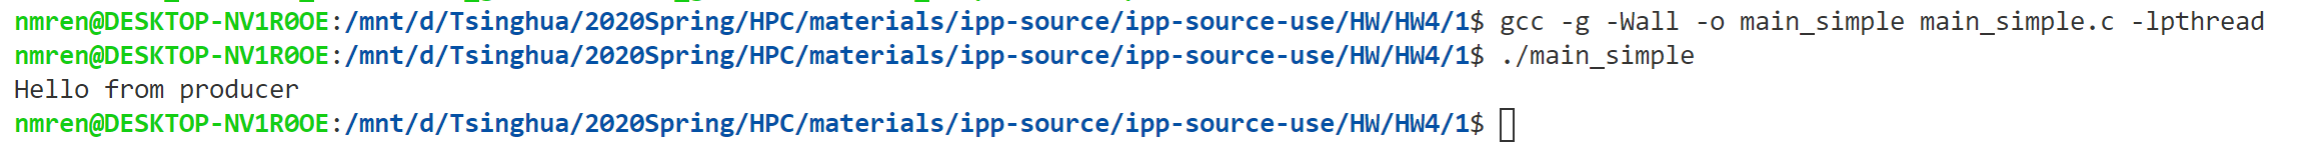
\includegraphics[width=\textwidth]{1simple.png}
        \caption{第1题第1小问实验结果}
    \end{figure}

\subsection{2k个线程生产者-消费者同步}
若想把上面双进程的生产者消费者同步推广到2k个进程之间,需要至少设置k个
\footnote{为了直接使用线程下标访问的便利性,下面的代码中事实上设置了2k个message\_available变量,只有下标为偶数的有用。}
message\_available变量来判断哪个进程可以打印消息。此外,还需要设置一个
控制写入的变量,以保证缓冲区不会在消息被对应的偶数号进程接受前,又被新的奇数号进程写入。线程函数代码如下:
\begin{lstlisting}[language={c}]
    int okToWrite = 1;
    void *Send_msg(void* rank) {
       long my_rank = (long) rank;
       while (1) {
          pthread_mutex_lock(&mutex);
          if (my_rank % 2 == 0) {
             if (message_available[my_rank]) {
                printf("%s, in consumer %ld\n", message, my_rank);
                okToWrite = 1;
                pthread_mutex_unlock(&mutex);
                break;
             }
          } else if (okToWrite) {
             sprintf(message, "Hello from producer %ld", my_rank);
             message_available[(my_rank + thread_count - 1) % thread_count] = 1;
             okToWrite = 0;
             pthread_mutex_unlock(&mutex);
             break;
          }
          pthread_mutex_unlock(&mutex);
       }
       return NULL;
    }  /* Send_msg */
    
    \end{lstlisting}

    实验结果如下:
    \begin{figure}[h]
        \centering
            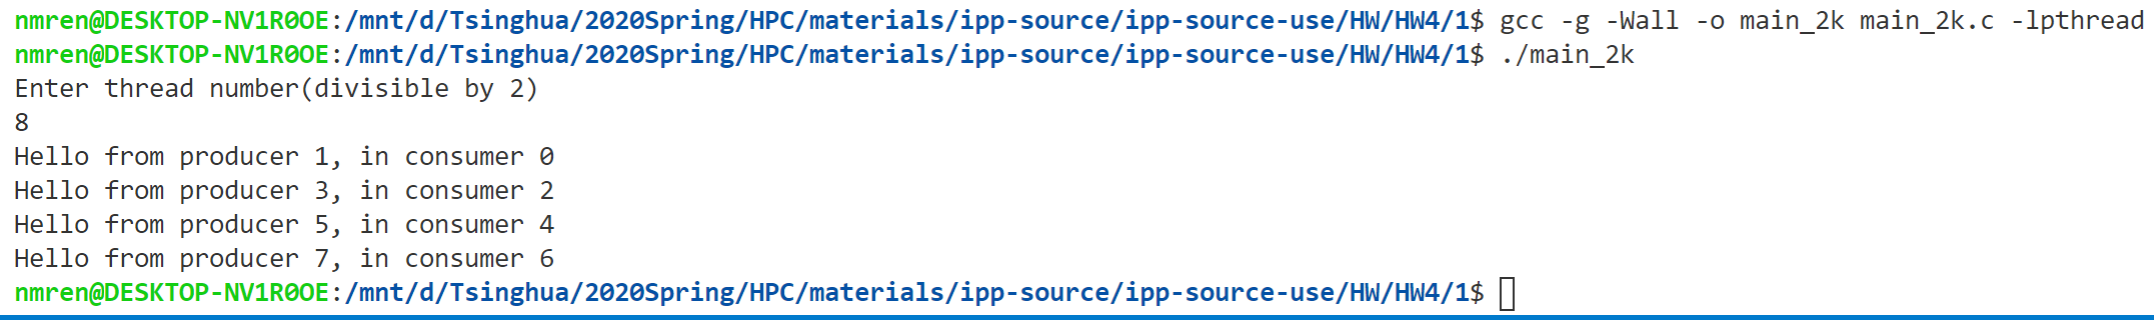
\includegraphics[width=\textwidth]{12k.png}
            \caption{第1题第2小问实验结果}
        \end{figure}


\subsection{每个线程既是消费者又是生产者}
对于更一般的情况,每个线程都是消费者和生产者,我们需要设立一个变量表示
缓冲区中目前有无未发送的消息,如果没有未被接收的消息,并且当前进入互斥锁的
线程没有发送过消息,则令其发送消息到缓冲区,并且使标记对应的线程可接收消息。如果有未被接受的消息,并且当前进入
互斥锁的线程可以接收消息了,则令其接收消息。对于已经既发送过消息也接受过消息的线程,我们使其调用break退出循环。
线程函数代码如下:


\begin{lstlisting}[language={c}]
    // indicates whether there're unreceived message in the buffer
    int messageBusy = 0; 
    void *Send_msg(void* rank) {
       long my_rank = (long) rank;
       while (1) {
          pthread_mutex_lock(&mutex);
          if (!messageBusy) {
             if (!sent[my_rank]) {
                sent[my_rank] = 1;
                sprintf(message, "Hello from %ld", my_rank);
                message_available[(my_rank + 1) % thread_count] = 1;
                messageBusy = 1;
                if (sent[my_rank] && recved[my_rank]) {
                   pthread_mutex_unlock(&mutex);
                   break;
                }
             }
          } else {
             if (message_available[my_rank]) {
                printf("%s, in %ld\n", message, my_rank);
                recved[my_rank] = 1;
                messageBusy = 0;
                if (sent[my_rank] && recved[my_rank]) {
                   pthread_mutex_unlock(&mutex);
                   break;
                }
             }
          }
          pthread_mutex_unlock(&mutex);
       }
    
       return NULL;
    }  /* Send_msg */
    
    
    \end{lstlisting}


    实验结果如下:
    \begin{figure}[h]
        \centering
            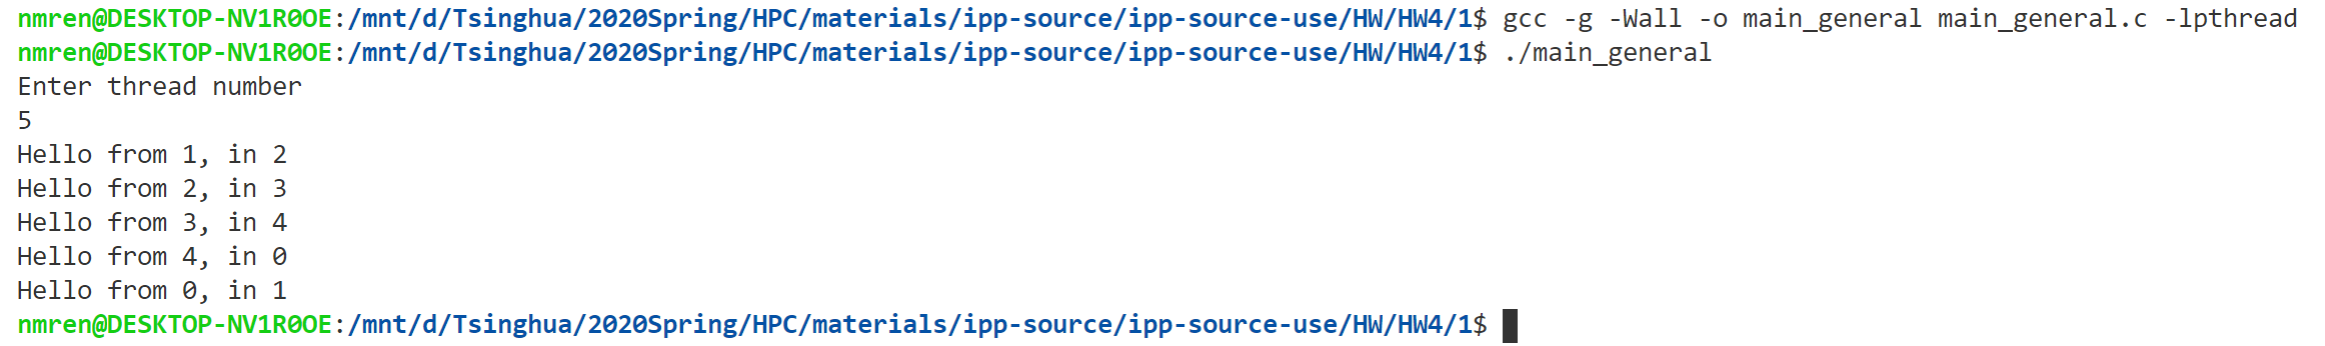
\includegraphics[width=\textwidth]{1general.png}
            \caption{第1题第3小问实验结果}
        \end{figure}


\section{第2题}
本题中给出了一系列链表操作,我将逐一指出其问题
\subsection{两个Delete操作同时执行}
如图4所示,如果同时执行删除2和5,理想的情况是head\_p的指针指向8,2和5直接被删除。
可能出现的一种错误情况是,head\_p的next指针指向了5,而2的next指针指向了8,这可能就会造成意想不到的错误。

\begin{figure}[h]
   \centering
       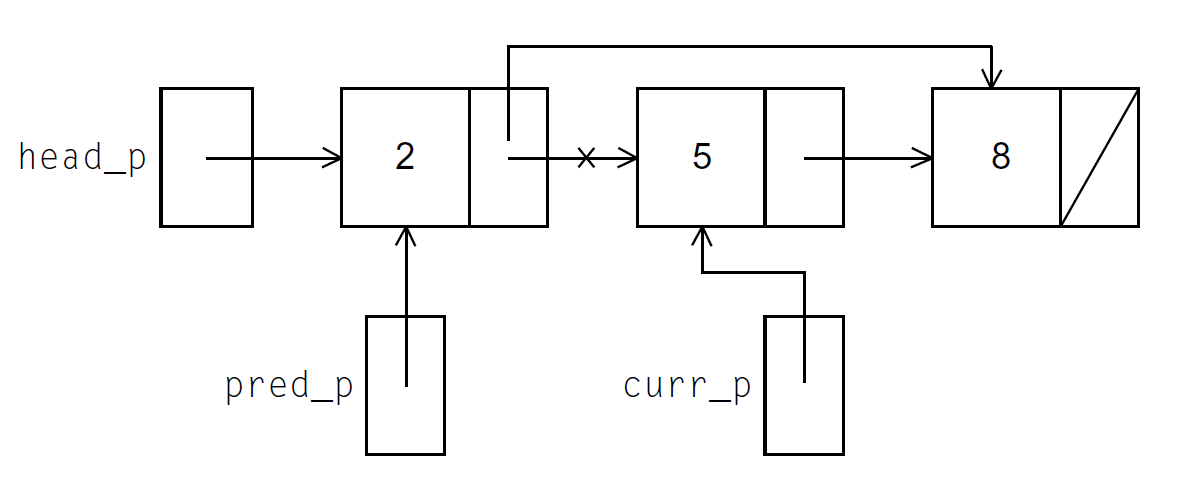
\includegraphics[width=0.7\textwidth]{21.png}
       \caption{删除链表中元素}
   \end{figure}

\subsection{一个Insert和一个Delete操作同时执行}
如图5所示,如果此时同时删除5和插入7,理想的情况是链表元素为head\_p, 2, 7, 8.
但可能出现的错误情况是:7正在将5作为自己的前继,并且此时5已经基本删除完毕,即2的next指针连接到8了,
这就造成了7的插入无效,这就可能造成一些意想不到的问题。

\begin{figure}[h]
   \centering
       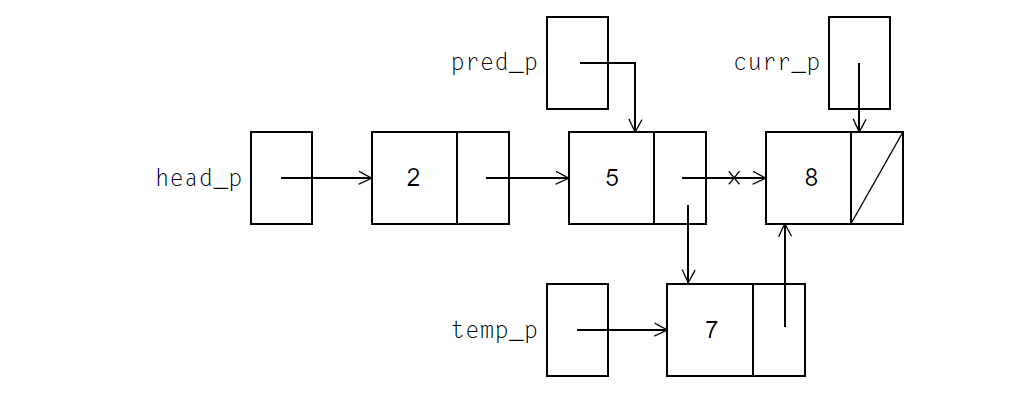
\includegraphics[width=0.7\textwidth]{22.png}
       \caption{插入一个元素}
   \end{figure}
\subsection{一个Member和一个Delete操作同时执行}
如图6所示,如果此时同时执行Member(5)和Delete(5),理想情况是
删除5成功并报告已经没有5了。可能造成的错误是,
报告了Member(5)报告5仍然存在,但是5已被删除。
这就可能造成一些意想不到的问题。

\begin{figure}[h]
   \centering
       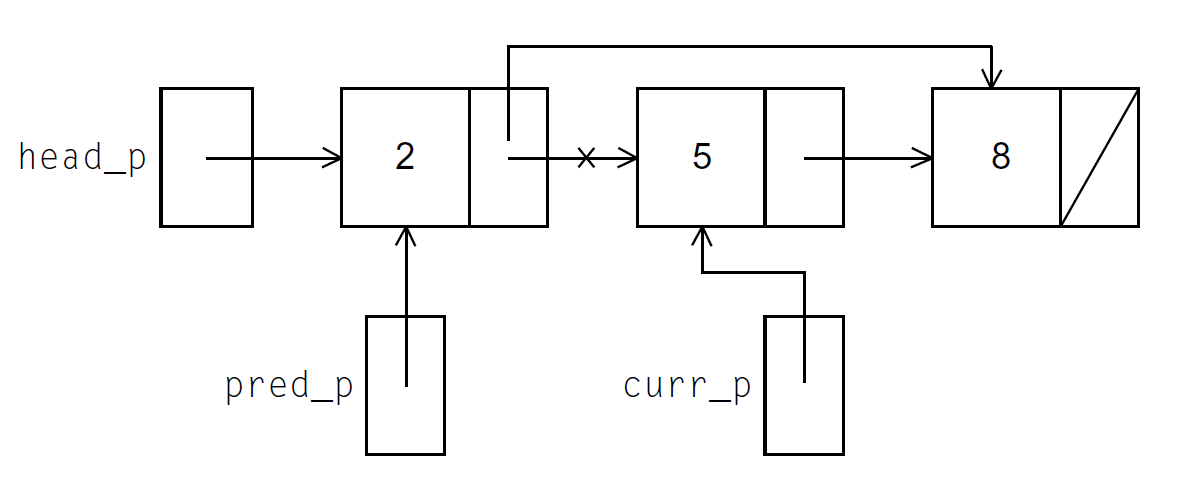
\includegraphics[width=0.7\textwidth]{21.png}
       \caption{删除链表中元素}
   \end{figure}

\subsection{两个Insert同时执行}
如图7所示,如果同时想插入6和7,理想情况是操作完毕后,
链表中元素为head\_p, 2, 5, 6, 7.但有可能出现的一种错误情况是,6先被插入到5和8之间,但是很快7也被插入到5和8之间,
并且5的后继被设定为了7,这样就会导致6的插入无效,链表中的元素变为head\_p, 2, 5, 7,这可能就会造成一些意想不到的问题。

\begin{figure}[h]
   \centering
       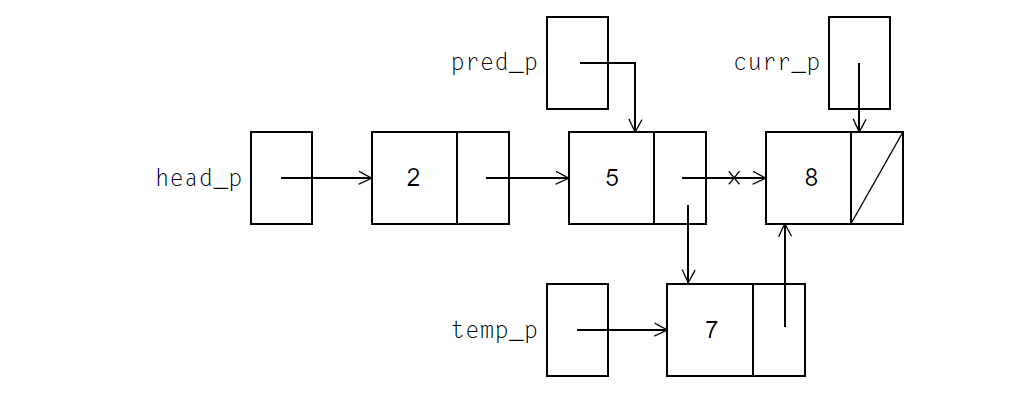
\includegraphics[width=0.7\textwidth]{22.png}
       \caption{插入一个元素}
   \end{figure}

\subsection{一个Insert和一个Member同时执行}
如图8所示,如果同时执行Insert(7)和Member(7),理想情况是
插入7成功并且报告有7.
一种可能错误的情况是Member(7)先执行并且报告没有7,但7已经被插入了。
这里就可能造成一些意想不到的问题。

\begin{figure}[h]
   \centering
       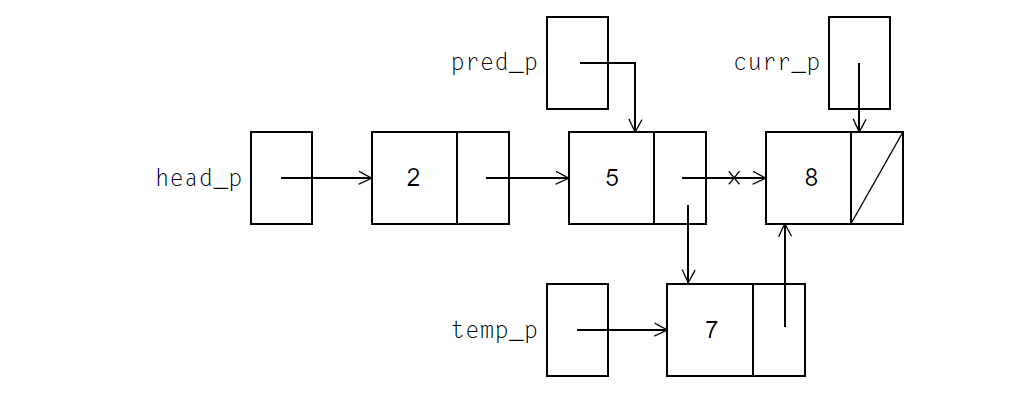
\includegraphics[width=0.7\textwidth]{22.png}
       \caption{插入一个元素}
   \end{figure}

\section{第3题}

这样做是不安全的,可能出现错误。如图9所示,如果同时插入3和删除5,在读的阶段两个操作不互斥,
则删除5和插入3操作的curr\_p都会指向5。在写的阶段,二者互斥,如果删除5先进行了,则5的指针就会被释放,
此时插入3,3的后继仍然会被设定为5,但5已经不存在了,3无法和后面的8连接上,这就会导致错误。

\begin{figure}[h]
   \centering
       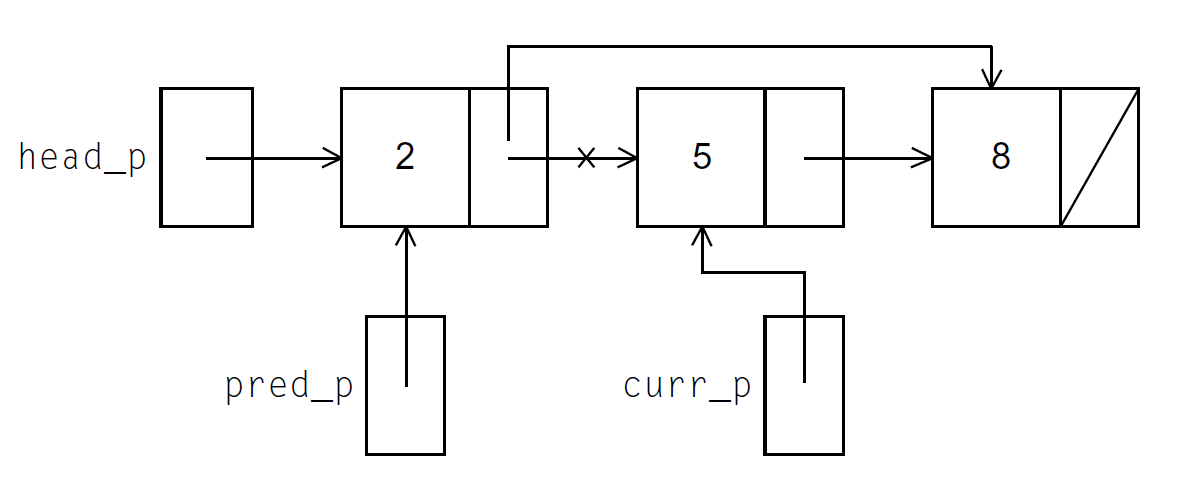
\includegraphics[width=0.7\textwidth]{21.png}
       \caption{删除链表中元素}
   \end{figure}

\section{第4题}
\subsection{解题思路}
本题需要在主线程创建任务队列,然后让新生成的线程去执行任务,在任务执行结束后结束所有线程并退出。我的主要思路如下:

首先在主线程内输入许多任务,放入一个队列里。
\footnote{这一步可以手动输入任务编号,也可以直接输入make check进行随机生成并与串行程序对拍。}
然后生成许多线程,在主线程没有开始逐个遍历任务时,生成的线程都需要挂起等待。
接下来主线程逐个循环任务,对于每个任务一次只会有一个线程执行,并且在这个线程执行完任务后,该线程
继续回到挂起等待任务的状态,主线程然后
才会遍历到下一个任务。当主线程的全部任务已经遍历完后,主线程通知其他线程结束任务并结束线程,释放内存等等。

这里有一些问题值得讨论。例如如何保证每个线程执行完任务后,主线程才可以
遍历到下一个任务。这个问题我是通过条件变量来解决的,我会在主线程的任务循环里
加入一个条件变量,只有每个线程执行完任务并发送信号后,主线程才能继续进行下一个任务循环。
此外,我还在线程函数中使用了条件变量,只有主线程发送信号时,才会有1个线程领取任务并执行,
当主线程发送broadcast信号并标记没有任务时,所有线程都会退出。这里需要注意的一个问题是,
当主线程发送broadcast信号并标记没有任务时,如果有线程正在执行任务,就可能无法正常退出。
我的解决方法是在条件等待前加入是否有任务的判断,如果没有任务了,正在执行前一个任务的线程
返回到条件等待前,就可以通过没有任务的判断退出。

本题的链表部分实现,主要参考了课本示例代码中ch4/linked\_list.c中的链表实现方式,线程的操作部分
均由我设计并实现。

\subsection{运行方式}
在目录下运行make即可进行编译。运行make run命令即可运行并行链表操作的程序,不过这种
运行方式需要手动输入任务序列以及输入链表的操作。更方便并且易于对比并行串行结果的运行方式
是输入make check, 该命令会自动调用check.py以及datamaker.py, 随机生成输入数据并通过对比
整个链表操作过程中的输出来验证正确性。具体参数如线程数、任务数在makefile中有对应变量可以更改,
若想更改任务数,需要将makefile和datamaker.py中的TASKS\_COUNT变量统一更改为1个值。
默认的任务数为60,线程数为10.
\subsection{测试结果}
使用10线程,15个任务随机输入,对拍2000余组数据均正确。

在本题中,我着实感受到了不同线程之间异步执行的复杂性,这需要非常周密的考虑和非常全面的测试。




\section{第5题}
\subsection{解题思路}
本题需要通过Pthreads的并行化方式,计算斐波那契数列第n项。我的思路如下。

斐波那契数列数列计算公式为$fib(n+2)=fib(n+1)+fib(n), fib(0)=0, fib(1)=1$.但是这样的公式不便于并行化,因为这样计算的话,每一项都依赖于前一项的结果,
这是一个典型的串行思路。因此我选择了另外一种计算斐波那契数列的等价公式,即:
$$   \left(\begin{array}{c}
      f_{n+1} \\
      f_{n}
      \end{array}\right)=\left(\begin{array}{cc}
      1 & 1 \\
      1 & 0
      \end{array}\right)\left(\begin{array}{c}
      f_{n} \\
      f_{n-1}
      \end{array}\right) \quad\left(\begin{array}{c}
      f_{n} \\
      f_{n-1}
      \end{array}\right)=\left(\begin{array}{cc}
      1 & 1 \\
      1 & 0
      \end{array}\right)^{n-1}\left(\begin{array}{c}
      f_{1} \\
      f_{0}
      \end{array}\right)
$$
由于$f_1, f_2$已知,我们只需要计算
$\left(\begin{array}{cc}
   1 & 1 \\
   1 & 0
   \end{array}\right)^{n}$
即可得到结果。注意到同一个矩阵的$n$次方的操作是可交换的,我们就可以利用这个性质,
使用类似全局求和的思路,
巧妙而简便地计算出$f_n$.

具体实现思路如下:首先输入线程数和要计算的项数,然后将待计算的项数尽量平均分配给每个线程。
之后在线程函数中,先令每个线程计算其分配到的局部矩阵乘方数,然后通过互斥锁,将局部的矩阵乘方结果乘到全局的矩阵
乘方结果上,待所有线程计算完毕后,在主线程中读取结果。

这里有个小问题需要注意,即主进程要在所有线程计算完毕后才能读取结果,否则会导致错误。
我的解决方式是:在主进程中加入循环,循环里放入条件变量,并且每个线程结束后发送信号,
只有当完成线程函数的线程数达到总线程数时,主线程才会继续进行。这样就可以保证所有线程计算时,
主线程不继续进行,只有所有线程计算完毕后主线程才可以继续进行。




\subsection{运行方式}

在5文件夹下运行make命令即可编译程序,make run命令即可运行程序,make check命令即可
随机生成输入数据,使程序进行对拍。

\subsection{结果分析}
对拍1000余组的数据,并行结果与串行结果均一致,保证了程序的正确性。
不过由于long long的数据范围较为有限,$fib(92)\approx7\times10^{18}$就已经接近溢出了,
因此在这样小的数据范围下,据我观察并行结果都要比串行结果慢很多。例如10线程计算$fib(92)$时,
并行计算时间约为$1.6\times10^{-5}s$, 串行计算时间为$1.2\times10^{-6}s$. 
同样,由于long long的数据范围有限,不便于做更大规模的测试。
\footnote{数值溢出时,并行与串行的结果也是一致的,并且较大范围内的数据下能够体现并行的
速度优势。例如20线程计算$fib(100000)$时,并行计算时间约为$5.1\times10^{-5}s$,串行时间
约为$3.8\times10^{-4}s$。但这样的测试可靠性有待商榷,因此不做详细分析。
}


\section{总结}
在本次实验中,我学习到了Pthreads编程的方法和技巧,也深刻地体会了多线程之间
异步执行的复杂性,锻炼了较为缜密的思维以及编程和调试的能力。感谢老师和助教给予的帮助!
%----------------------------------------------------------------------------------------

\bibliographystyle{plain}
\bibliography{ref} %这里的这个ref就是对文件ref.bib的引用

\end{document}
